The implementation of this program prioritises scale-ability and maintenance. This meant comments, logic separated out into classes, and appropriate data structures or design patterns used. \\

\vspace{.2cm}
As a result, there are 7 different classes in this program. \\

\begin{table}[!ht]
    \centering
    \begin{tabular}{l p{12cm}} \midrule
        \textbf{Class} & \textbf{Description} \\ \midrule
        Client & The main class of the program that controls the overall flow of the system. \\ \midrule
        Connection & An abstract class for communication with the ds-sim server from anywhere in the program \\ \midrule
        Algorithm & An interface for all algorithms \\ \midrule
        AlgorithmFactory & Where algorithms are requested and created from \\ \midrule
        LRRAlgorithm & A class providing the functionality of the LRR algorithm job scheduling \\ \midrule
        Server & Stores the base and current details of servers, based on the data provided by the ds-server \\ \midrule
        Job & Stores the base and current details of jobs, based on the data provided by the ds-server \\ \midrule
    \end{tabular}
\end{table}

\subsection{Arguments}
To connect to the ds-sim server the correct host and ports needs to be used. To make use of the ds-sim server, the client also needs to be able to run an algorithm to handle the job scheduling. Therefore the client has required arguments to determine these variables, provided in the order `hostname` `port` `algorithm`. If any of these are missing then the client won't run. However if the algorithm doesn't match to any in the program then it defaults to LRR, since this was the first (and only) implemented algorithm. The suggested host is localhost and the suggested port is 50000, since these are the defaults for ds-sim.


\subsection{Connection and Communication}
There is a single class in charge of all connection and communication between the client and the server, called Connection. This class was made static so that any part of the program could use a unified method for communication, guaranteeing that they use the same socket and message format (a byte array ending in a newline). The Socket comes from the java.net library, and messages sent or received use the DataOutputStream and BufferedReader classes from the java.io library. \\

\vspace{.2cm}
Once the initial arguments have been verified they are given to Connection. Connection then proceeds to connect to the socket and initialise communication. However this is \textit{not} where authentication is done, since that is logic determined by the main class. Only after the connection has been initialised will the Client authenticate the connection by sending the HELO and AUTH commands to ds-server. \\

\vspace{.2cm}
At the end of the program, once all communication with the server has been completed (i.e. the server has sent "NONE" indicating there are no more jobs to be received), the client asks Connection to gracefully close the connection by sending a "QUIT" message to the server. Then, the program ends.

\newpage
\subsection{Algorithms and Scheduling}
As mentioned, the client must be able to select an algorithm based on the corresponding value provided in the args. Currently the only valid algorithm names are 'lrr' or 'LRR' - case has been ignored here. Any other algorithms requested will default to LRR. \\ 

\vspace{.2cm}
Algorithms are created as classes designed with the Factory pattern. The client uses the abstract class AlgorithmFactory to generate the algorithm required, hidden behind the Algorithm interface. This makes the code incredibly easy to modify without adjusting existing code. When a new algorithm is added, only two things need to be done. First, a new class implementing Algorithm needs to be created and the scheduleJob function designed. Secondly, the algorithm needs to be added to the AlgorithmFactory so that it can actually be used. \\

\vspace{.2cm}
The diagram below demonstrates how the Factory pattern was implemented. Note that "OtherAlgorithm" is not an existing algorithm class, and is simply here for demonstration purposes.
\begin{center}
    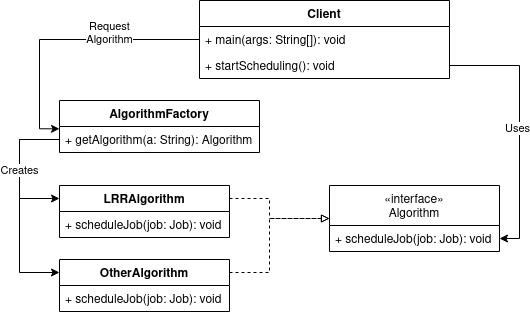
\includegraphics[scale=.7]{AlgorithmFactory.png}
\end{center}

After the connection with the server has been established and authenticated, the client starts taking data from the server and scheduling jobs. At the current stage, the only messages the server will send are "JOBN" (send a job), "JCPL" (complete a job), or "NONE" (no jobs left). If "JOBN" is called, a new Job will be created using the data provided by the ds-server and it will be sent as a parameter into the Algorithm's scheduleJob function. Then the client requests more jobs by sending "REDY". If "JCPL" is sent, the client tells the stored server holding the job that it's complete so that it can be marked complete. Then the client sends "REDY", requesting data again. If "NONE" is sent, the server has no more jobs to schedule.

\subsection{Largest Round Robin Algorithm}
\vspace{.2cm}
Each Algorithm takes in a Job that needs completing. In the LRR Algorithm, a request is sent to ds-server to return all servers that are capable of handling the job. A list of servers will be returned, and these are stored in the client's HashMap of types String (key) and Server (value). If the servers already exist in the hashmap, they will have variables such as "currentMemory" updated so that both base and current values can be accessed. \\

\vspace{.2cm}
Finally, the largest server needs to be chosen. It is simply picked based on which of the available servers has the the largest number of CPU cores, and picking the first one if there are multiple available. However, servers are not simply identified by a name but also have an id (e.g. Server 0, Server 1, AnotherServer 0, AnotherServer 2). Once largest server identified it picks the server id that has had the least number of jobs assigned to it. \\

\vspace{.2cm}
Finally, the algorithm schedules the job by sending a "SCHD" command through Connection.